%%%%%%%%%%%%%%%%%%%%%%%%%%%%%%%%%%%%%%%%%%%%%%%%%%%%%%%%%%%%%%%%%%%%%%%%%%%%%%%
%%%%%%%%%%%%%%%%%%%%%%%%%%%%%%%%%%%%%%%%%%%%%%%%%%%%%%%%%%%%%%%%%%%%%%%%%%%%%%%
%%%%%%%%%%%%%%%%%%%%%%%%%%%%%%%%%%%%%%%%%%%%%%%%%%%%%%%%%%%%%%%%%%%%%%%%%%%%%%%
%%%%%%%%%%%%%%%%%%%%%%%%%%%%%%%%%%%%%%%%%%%%%%%%%%%%%%%%%%%%%%%%%%%%%%%%%%%%%%%
\chapter{Results of Network Analysis}
\label{ch:results}
%%%%%%%%%%%%%%%%%%%%%%%%%%%%%%%%%%%%%%%%%%%%%%%%%%%%%%%%%%%%%%%%%%%%%%%%%%%%%%%
%%%%%%%%%%%%%%%%%%%%%%%%%%%%%%%%%%%%%%%%%%%%%%%%%%%%%%%%%%%%%%%%%%%%%%%%%%%%%%%
%%%%%%%%%%%%%%%%%%%%%%%%%%%%%%%%%%%%%%%%%%%%%%%%%%%%%%%%%%%%%%%%%%%%%%%%%%%%%%%
%%%%%%%%%%%%%%%%%%%%%%%%%%%%%%%%%%%%%%%%%%%%%%%%%%%%%%%%%%%%%%%%%%%%%%%%%%%%%%%
This chapter summarizes the analysis results of the temporal, spatial proximity network of honey bees, consisting of three consecutive time-aggregated snapshots.\\
The first section describes results related to static aspects of one snapshot~3.
I investigate the snapshot on three levels.First I examined the networks global structure and derived properties of the overall colony (global level). Second I studied the characteristics of individual bees (local level), and its relation to detection frequency and age.
Additionally, I investigated the intermediate level of the colonies social organization by detecting communities and inspecting their practical meaning.\\
The second section focuses on the temporal network aspects of all three snapshots.
I investigated the stability of local and global properties, as well as the stability of functional groups of bees concerning age and spatial distribution. Furthermore, the dynamics of individual bees regarding their group membership over time is examined.
The last section fo this chapter summarizes the main results and discusses the findings.

%%%%%%%%%%%%%%%%%%%%%%%%%%%%%%%%%%%%%%%%%%%%%%%%%%%%%%%%%%%%%%%%%%%%%%%%%%%%%%%
%%%%%%%%%%%%%%%%%%%%%%%%%%%%%%%%%%%%%%%%%%%%%%%%%%%%%%%%%%%%%%%%%%%%%%%%%%%%%%%
\section{Static Perspectives of Honey Bee Networks}
%%%%%%%%%%%%%%%%%%%%%%%%%%%%%%%%%%%%%%%%%%%%%%%%%%%%%%%%%%%%%%%%%%%%%%%%%%%%%%%
%%%%%%%%%%%%%%%%%%%%%%%%%%%%%%%%%%%%%%%%%%%%%%%%%%%%%%%%%%%%%%%%%%%%%%%%%%%%%%%

TODO write some intro

I analyzed a temporal network, consisting of three time-aggregated snapshots; these are referred to below as snapshot~1~($N=922$), snapshot~2~($N=978$) and snapshot~3~($N=922$). 
The snapshots are aggregated for ten hours (108,000 frames) starting at 8~a.m. and lasting until 6~p.m, see table~\ref{tab:networks} for details about the added bees per day,  figure~\ref{fig:ages} for the age distributions. Figure~\ref{fig:network-matching} shows the proportion of intersecting bees between each snapshot. This figure illustrates the stability of the network concerning its size. 

\begin{table}
\centering
\caption[Sampling period]{\textbf{Sampling period} Overview of the chosen day networks including the number of added bees and the time they were added to the hive.}
\vspace*{5mm}
\begin{tabularx}{\textwidth}{ccccccc}
\toprule
{} & 20.08.16 & 21.08.16 & 22.08.16 & 23.08.16 & 24.08.16 \\
\midrule
Network ID & 1 & - & 2 & - & 3 & \\
Number of added bees & 0 & 0 & 110 & 60 & 0 \\
Time added & - & - & 2~p.m. & 6~p.m. & - \\
\bottomrule
\end{tabularx}
\label{tab:networks}
\end{table}

\begin{figure}[htb]
	\centering
	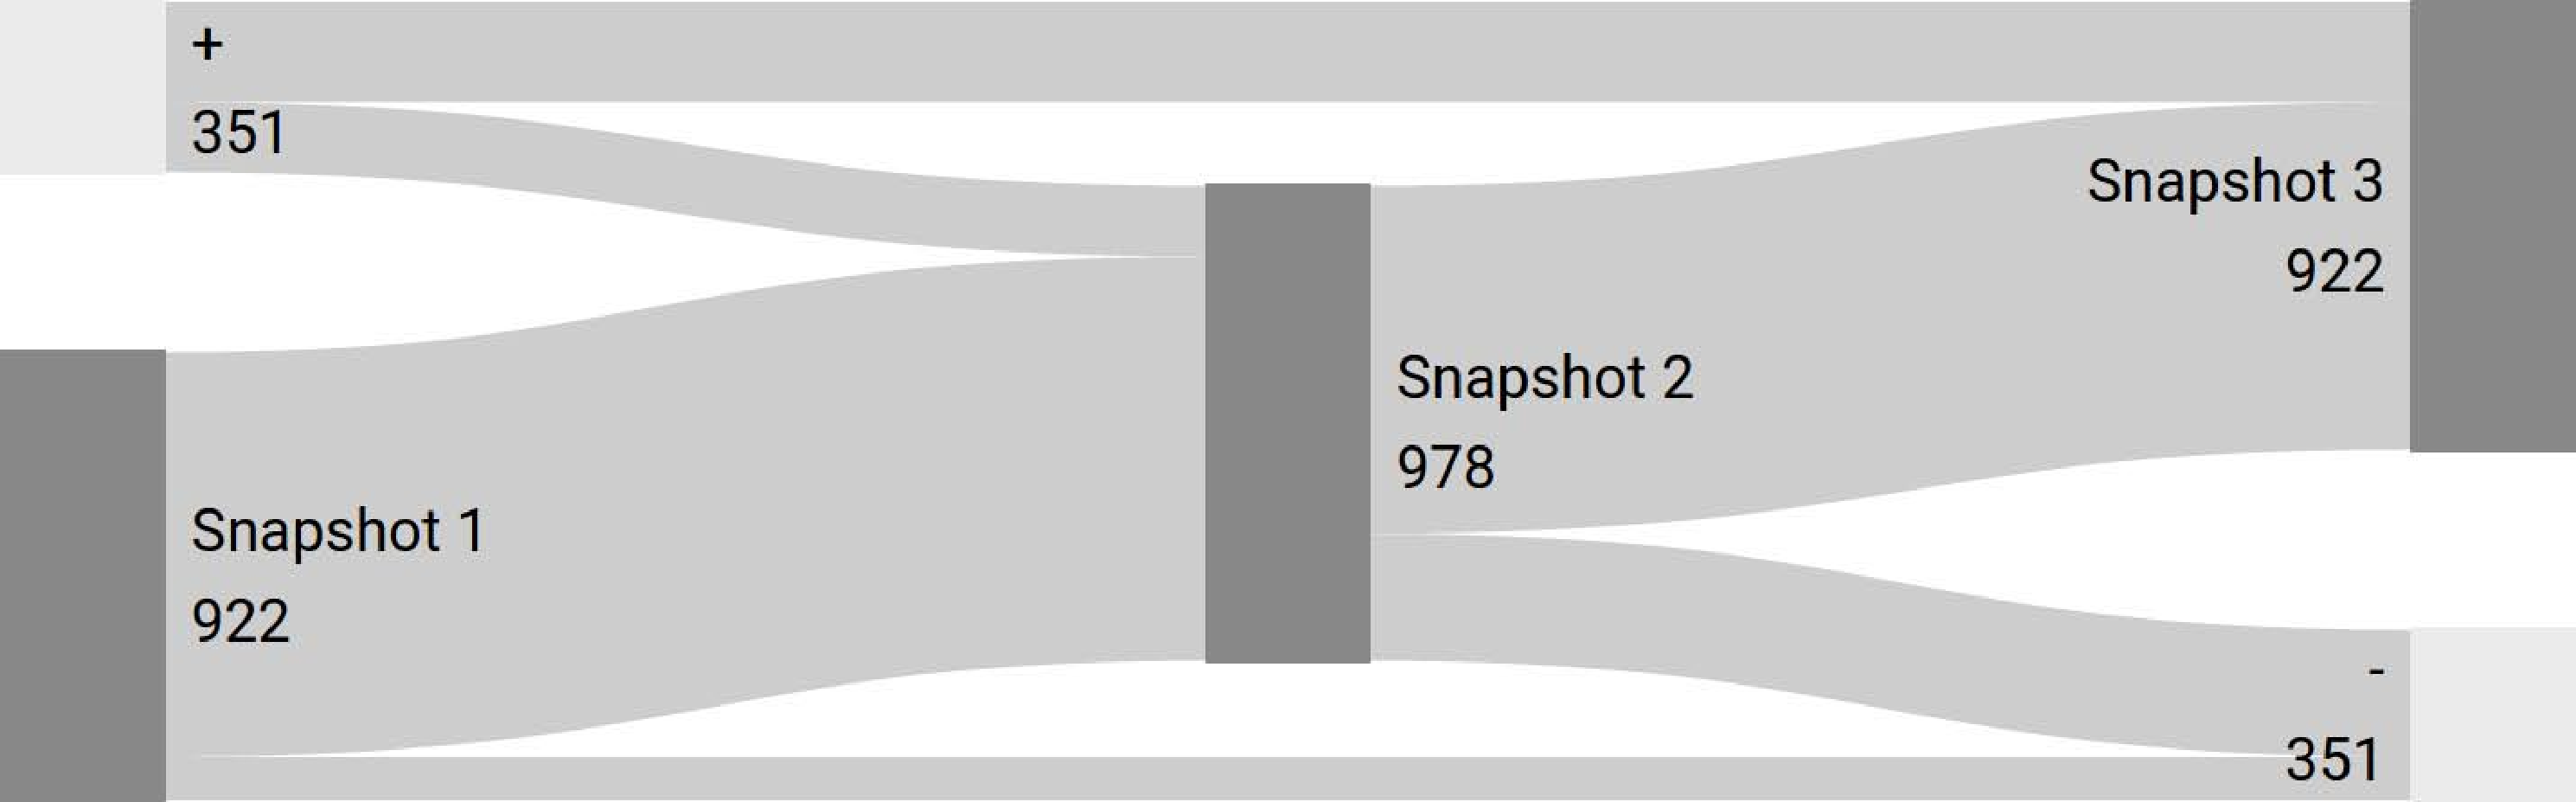
\includegraphics[width=.8\textwidth]{Figures/network_matching}
	\caption[Number of bees per snapshot]{\textbf{Number of bees per snapshot} This figure show the amount of bees for each snapshot and the proportion of intersecting bees between snapshots.}
	\label{fig:network-matching}
\end{figure}

%%%%%%%%%%%%%%%%%%%%%%%%%%%%%%%%%%%%%%%%%%%%%%%%%%%%%%%%%%%%%%%%%%%%%%%%%%%%%%%
\subsection{Properties of the Bee Colony}
\label{subsec:colony}
%%%%%%%%%%%%%%%%%%%%%%%%%%%%%%%%%%%%%%%%%%%%%%%%%%%%%%%%%%%%%%%%%%%%%%%%%%%%%%%
Each snapshot consists of one component.
The density $D$ is over 50\% for all snapshots (69\%; 54\%; 61\%).
The diameter $\langle d_{\texttt{max}} \rangle$ is $3$ and the average shortest path length $\langle d \rangle$ is inbetween $1$ and $2$.
The global clustering coefficient $C_\Delta$ of all snapshots is higher than compared to an Erd\H{o}s-R\'{e}niy random graph, averaged over 100 runs using the same number of nodes and edges.
On average, each bee is connected to at least 50\% of the colony (68\%; 52\%; 61\%). During the ten hour observation peroid a bee interacts on average over $4,000$ times ($5,680$; $3,978$; $4,206$)
Table~\ref{tab:stats} summarizes those basic network properties for each snapshot and lists the values of its corresponding random graph.


Figure~\ref{fig:n3ageDist} shows the age distribution of the further investigated snapshot 3. This distribution corresponds to the artificial tagging of the bees. Consequently, bees of certain age groups are simply not present. The detection frequency of an individual bee is negatively correlated with its age (figure~\ref{fig:n3detfVSage}).

\begin{table}[htbp]
\small
\centering
\caption[Global network properties]{\textbf{Global network properties} $N$ number of nodes, $L$ number of links, $D$ diameter, $\langle d_{\texttt{max}} \rangle$ average path length, $\langle d \rangle$ diameter, $C_\Delta$ global clustering coefficient, $\langle k \rangle$ average degree and $\langle s \rangle$ represents the average strength, as introduced in section~\ref{sec:definitions}.}
\label{tab:stats}
\vspace*{5mm}
\begin{tabular}{rccccccccc}
\toprule
{} &  $N$ &   $L$ &  $D$ &  $\langle d_{\texttt{max}} \rangle$ &  $\langle d \rangle$ &   $C_\Delta$ & $\langle k \rangle$ &  $\langle s \rangle$ \\
\midrule
Snapshot 1 & 922 & 291179 & 0.69 & 3 & 1.32 &  0.79 & 631.62 & 5680.17 \\
Random 1  & 922 & 291179 & 0.69 & 2 & 1.31 &  0.69 & 631.62 & - \\ \midrule
Snapshot 2 & 978 & 256066 & 0.54 & 3 & 1.46 &  0.72 & 523.65 & 3977.94 \\
Random 2  & 978 & 256066 & 0.54 & 2 & 1.46 &  0.54 & 523.65 & - \\ \midrule
Snapshot 3 & 922 & 259421 & 0.61 & 3 & 1.39 &  0.75 & 562.74 & 4205.99 \\
Random 3  & 922 & 259421 & 0.61 & 2 & 1.39 &  0.61 & 562.74 & - \\
\bottomrule
\end{tabular}
\end{table}

The edge weight distribution is shown in figure~\ref{fig:edgeWdist}.
Most edges have a low weight; only a few edges have a high weight.
It seems that bees do not prefer individuals bees for interaction.[TODO. figure out what it means.]

\begin{figure}[bp]
	\centering
	\begin{subfigure}[b]{1\textwidth}
	\centering
	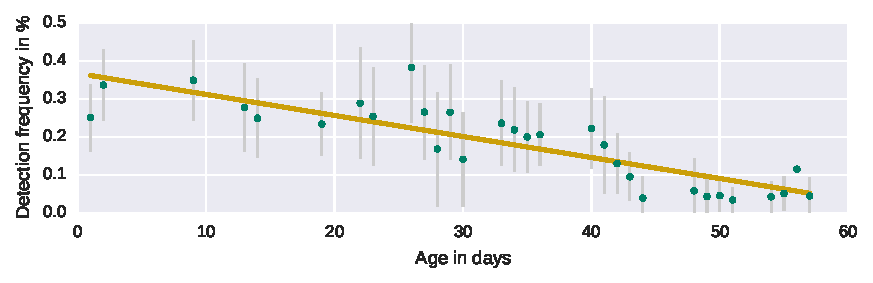
\includegraphics[width=1.0\textwidth]{Figures/n3_detFvsAge}
	\caption[Correlation]{Correlation}
	\label{fig:n3detfVSage}
	\end{subfigure} 
	\begin{subfigure}[b]{1\textwidth}
	\centering
	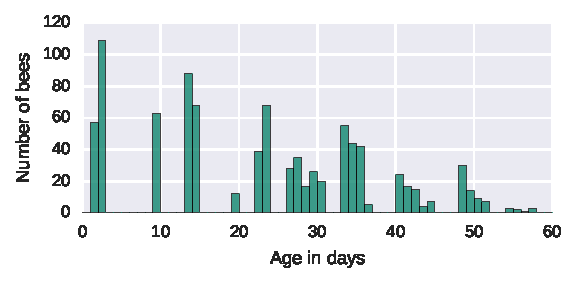
\includegraphics[width=1.0\textwidth]{Figures/n3_ages.pdf}
	\caption[Age distribution]{Age distribution}
	\label{fig:n3ageDist}
	\end{subfigure}
	\caption[Age distribution and correlation with detection frequency of snapshot~3]{\textbf{Age distribution and correlation with detection frequency of snapshot~3} (a) Detection frequency and the age of a bee seem to be negatively correlated. (b) The age of bees ranges from one to 60 day, but some age groups are missing.}
	\label{fig:ageDetF}
\end{figure}

\begin{figure}[htb]
	\begin{subfigure}[b]{0.49\textwidth}
	\centering
	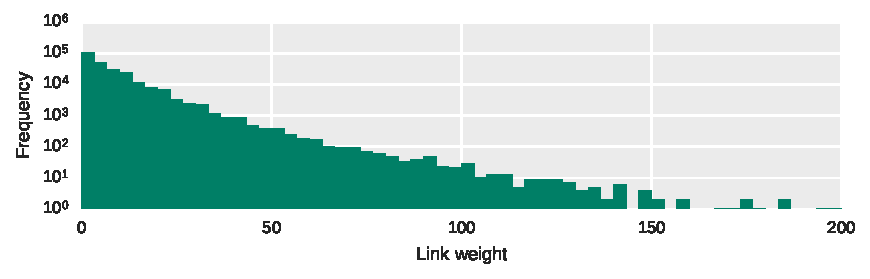
\includegraphics[width=1.0\textwidth]{Figures/n3-edgeWeightDist.pdf}
	\caption[Edge weight distribution]{Edge weight distribution}
	\label{fig:edgeWdist}
	\end{subfigure}
	\caption[Edge wights]{\textbf{Edge wights} (a) Correlation between number of interactions and total duration of interactions. The number of interactions is chose as the edge weight. (b)  The edge weight distribution decays exponentially.}
	\label{fig:edges}
\end{figure}
\clearpage
%%%%%%%%%%%%%%%%%%%%%%%%%%%%%%%%%%%%%%%%%%%%%%%%%%%%%%%%%%%%%%%%%%%%%%%%%%%%%%%
\subsection{Characteristics of Bees}
\label{subsubsec:bees}
%%%%%%%%%%%%%%%%%%%%%%%%%%%%%%%%%%%%%%%%%%%%%%%%%%%%%%%%%%%%%%%%%%%%%%%%%%%%%%%
For snapshot~3, I inspected the properties of each honey bee, concerning its degree~$k$, strength~$s$, local clustering coefficient~(lcc)~$c$, betweenness centrality~$C_B$ and closeness centrality~$C_C$ and derived charctersitics and properties of the honey bee colony.

\subsubsection{Low Hierarchical Structure}
The degree is normally distributed (a in figure~\ref{fig:n3-degreeStrLCC}).
Therefore most bees bee have the same high number of interaction partners.
The absence of hubs, a small number of highly connected bees, indicates a low hierarchical structure of the network.
Strength and lcc are also normally distributed (d and g in figure~\ref{fig:n3-degreeStrLCC}).
That also shows the absence of extreme values and confirms that bees are similar to each other regarding those properties.
Betweenness and closeness centrality (j and m in figure~\ref{fig:n3-degreeStrLCC}) also follow a normal distribution.
This leading to the assumption that no central or important bees exist.
All bees are similarly close to all other bees in the network, and every bee can reach any other bee with a few steps.
That also corresponds to the low average path length, and the small diameter of the network described in section~\ref{subsec:colony}.
The absence of bees with a high betweenness suggests that the colonies functionality is robust concerning the disappearance of single individuals.

\subsubsection{Local Network Measures and Detection Frequency}
Degree, strength, closeness and betweenness (b, e, k, and n in figure~\ref{fig:n3-degreeStrLCC}) show a positive correlated with the detection frequency. A low value corresponds to a low detection frequency. In contrast, the local clustering coefficient (h in figure~\ref{fig:n3-degreeStrLCC}) and detection frequency are negatively correlated.

\subsubsection{Local Network Measures and Age of Bees}
The histograms of degree, strength, betweenness, and closeness show a normal distribution with a tendency for bimodality. The local clustering coefficient distribution is instead right skewed, with one peak at $0.75$

There is no clear border between groups in the degree distribution plot (a), but a value around 0.4 can be estimated.
The strength histogram (d) seems to have a border at 1000.
For closeness (j) and betweenness (m), a border can be seen at 0.6 and 0.0001.
All distributions indicate a small group (~100 bees) and a second larger group containing the rest of the colony.

The first small group interacts on average with 20\% of the colony and has a very low strength (number of total interactions below 250). The closeness value is compared to the second group smaller but still over 0.5. The betweenness has a small range and is close to 0 for the first smaller group.
The second group interacts with about 80\%, corresponding to almost the entire colony and an average strength of 5000. A high strength can result from lots of neighbors with low edge weights or a few neighbors with high edge weight. The second is rather unlikely, looking at the edge weight distribution (figure~\ref{fig:edgeWdist}). The second group is characterized by a very high closeness (0.75) and a still very low betweenness but higher than the first group (0.0005).

All age-correlation plot show a seperate group of bees older than 45 days, seeming to correspond to the first smaller group of bees described above.
This older group is characterized by a low degree, a low strength, and low closeness and betweenness. In contrast, a high lcc, compared to the younger group is noticeable.
The younger group relates to a high degree and strength, as well as a high betweeness and closeness compared to the first group, but a lower lcc.
A high lcc of the old group indicates a high connectivity within the younger group and less connectivity between bees of the older group.

\begin{figure}[!h]
	\centering
	\begin{subfigure}[b]{1.0\textwidth}
	\centering
	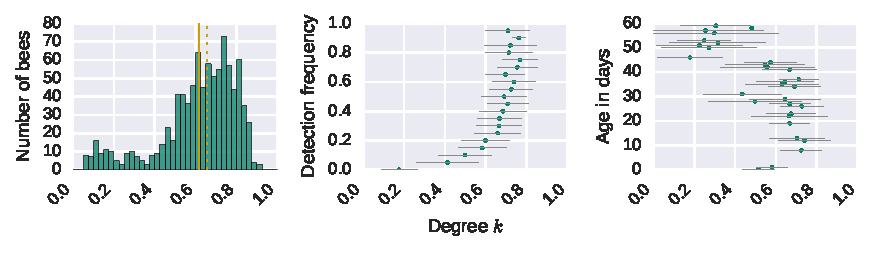
\includegraphics[width=1.0\textwidth]{Figures/n3-stat-degreeAgeDetF.pdf}
	%\caption[Degree]{\textbf{Degree}}
	%\label{fig:n3-degree}
	\end{subfigure}
	\begin{subfigure}[b]{1.0\textwidth}
	\centering
	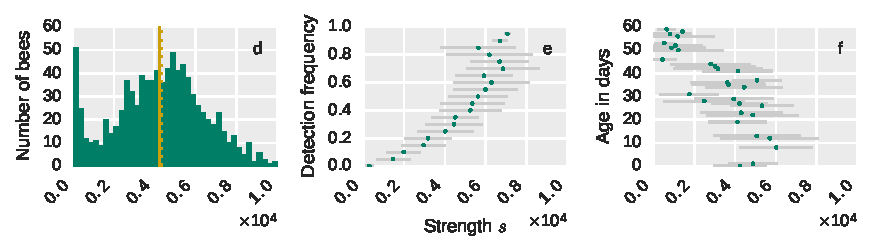
\includegraphics[width=1.0\textwidth]{Figures/n3-stat-strengthAgeDetF.pdf}
	%\caption[Strength]{\textbf{Strength}}
	%\label{fig:n3-strength}
	\end{subfigure}
	\begin{subfigure}[b]{1.0\textwidth}
	\centering
	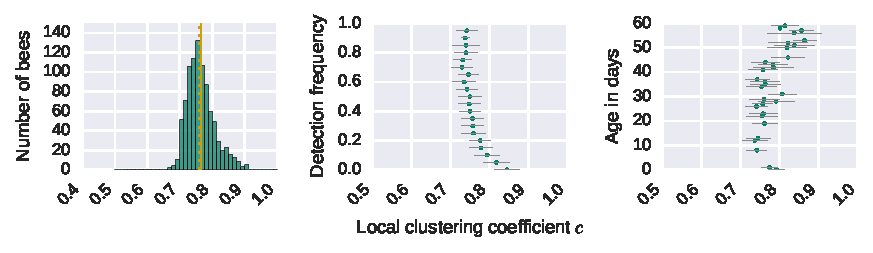
\includegraphics[width=1.0\textwidth]{Figures/n3-stat-lccAgeDetF.pdf}
	%\caption[Local clustering coefficient]{\textbf{Local clustering coefficient}}
	%\label{fig:n3-lcc}
	\end{subfigure}
	\begin{subfigure}[b]{1.0\textwidth}
	\centering
	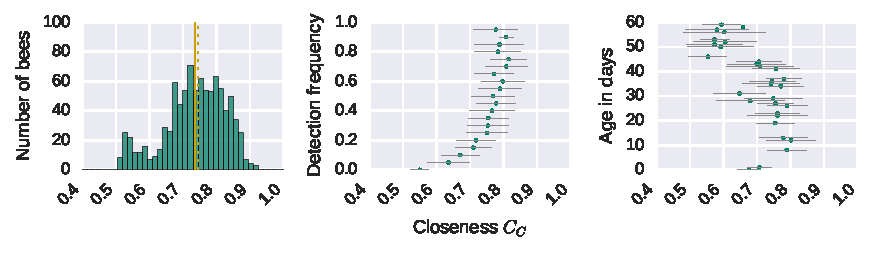
\includegraphics[width=1.0\textwidth]{Figures/n3-stat-closenessAgeDetF.pdf}
	%\caption[Closeness Centrality]{\textbf{Closeness Centrality}}
	%\label{fig:n3-closeness}
	\end{subfigure}
	\begin{subfigure}[b]{1.0\textwidth}
	\centering
	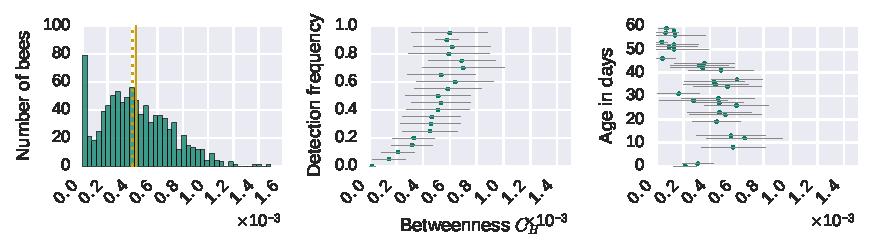
\includegraphics[width=1.0\textwidth]{Figures/n3-stat-betweenAgeDetF.pdf}
	%\caption[Betweeness Centrality]{\textbf{Betweeness Centrality}}
	%\label{fig:n3-between}
	\end{subfigure}
	\caption[Local measures in relation to age and detection frequency]{\textbf{Local measures in relation to age and detection frequency}}
	\label{fig:n3-degreeStrLCC}
\end{figure}
\clearpage
%%%%%%%%%%%%%%%%%%%%%%%%%%%%%%%%%%%%%%%%%%%%%%%%%%%%%%%%%%%%%%%%%%%%%%%%%%%%%%%
\subsection{Functional Groups within the Colony}
%%%%%%%%%%%%%%%%%%%%%%%%%%%%%%%%%%%%%%%%%%%%%%%%%%%%%%%%%%%%%%%%%%%%%%%%%%%%%%%

The leading eigenvector (LE) community detection algorithms revealed two communities with a similar size (modularity score of 0.25). The walktrap algorithm (WT) discovered three communities instead, also evenly distributed (modularity score of 0.23). Table~\ref{tab:n3-communities} lists the precise number of members per community and algorithm for snapshot~3.

For both algorithms the communities correspond to different age groups. For LE, the average age of the young community is $13.2$ days, and for the old community $28.7$ days. For WT, the average age of the young community is $6.6$ days and $29.3$ days for the older commmunity. The third middle-aged community of WT is on average 25.1 days old. The age distribution for each algorithm is represented in figure~\ref{fig:n3ageLE} and~\ref{fig:n3ageWT}. The two sample Kolmogorov-Smirnov test confirmed that the age distributions per community are significantly different. The corresponding $p$-values are listed in table~\ref{tab:n3-pvalues2}.

Each community occupies a different region of the comb.
Figure~\ref{fig:n3-communities} shows that the young communities spend the most time in the comb center and the old communities closer to the hive exit. The middle-aged community is positioned between the young and old community and in the periphery of the comb.

\begin{table}[htb]
\small
\centering
\caption[Communities per algorithm]{\textbf{Communities per algorithm} Communities marked with * contain the queen. Age and standard deviation (SD) are measured in days. The queen and nine bees with a negative age are excluded from this analysis.}
\label{tab:n3-communities}
\vspace*{5mm}
\begin{tabular}{lcrrrrr}
	\toprule
	{}  & Community ID & Members & Proportion & Age & SD\\
	\midrule  
	\quad LE  & CY & $*381$  & 41.78\% & $13.15$ & $\pm13.50$ \\
	          & CO & $531$   & 58.22\% & $28.70$ & $\pm11.67$ \\
    \midrule 
	\quad WT & CY & $*229$  & 25.11\% & $6.55$  & $\pm10.36$\\
			 & CM & $298$  & 32.68\% & $25.08$ & $\pm11.97$\\
			 & CO & $385$  & 42.21\% & $29.29$ & $\pm11.44$\\
	\bottomrule
\end{tabular}
\end{table}
\begin{table}[htb]
\small
\centering
\caption[Kolmogorov-Smirnov test]{\textbf{Kolmogorov-Smirnov test} $p$-values for leading eigenvector (LE) and walktrap (WT)}
\label{tab:n3-pvalues2}
\vspace*{5mm}
\begin{tabular}{crrrrr}
	\toprule
	 Communities & LE p-value & WT p-value\\
	\midrule 
    CY, CO & 5.10e-66 & 5.51e-67\\
    CY, CM &          & 1.10e-95\\
    CM, CO &          & 1.98e-05\\ 
	\bottomrule
\end{tabular}
\end{table}

\begin{figure}[!htb]
	\centering
	\begin{subfigure}[b]{1.0\textwidth}
	\centering
	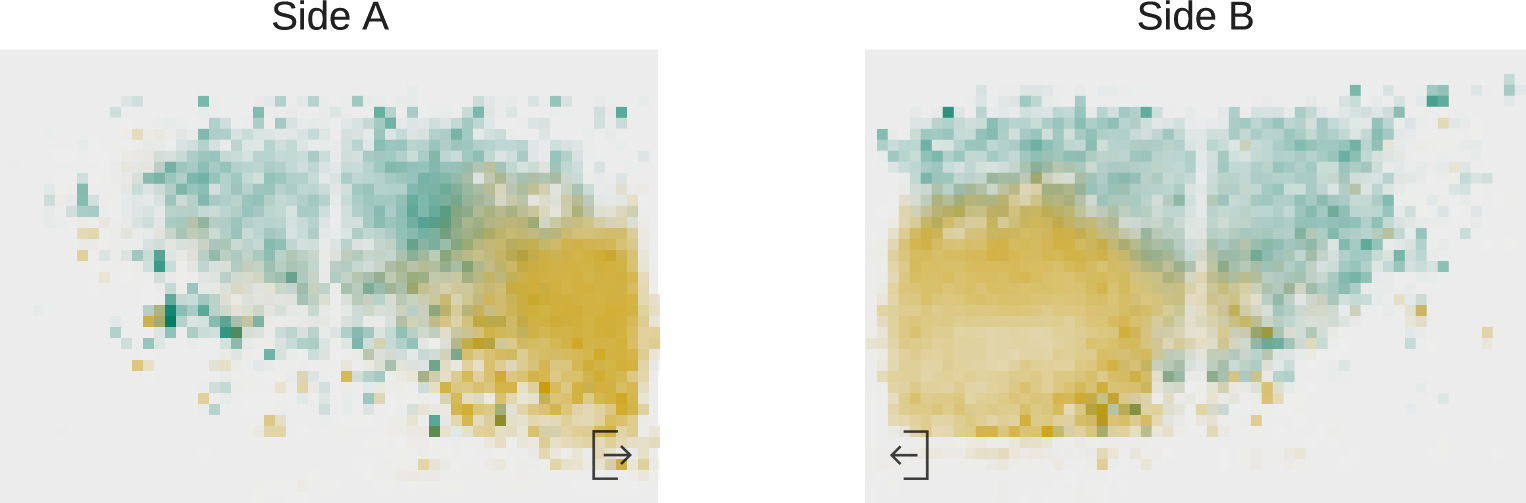
\includegraphics[width=1.0\textwidth]{Figures/le_network3}
	\end{subfigure}
	
	\begin{subfigure}[b]{1.0\textwidth}
	\centering
	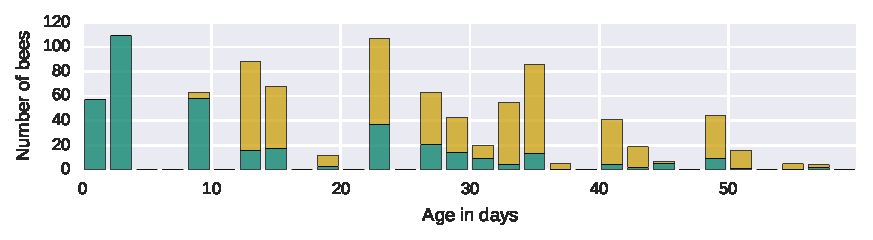
\includegraphics[width=1.0\textwidth]{Figures/n3-ageDistribution-LE}
	\caption[Leading eigenvector communities]{Leading eigenvector communities}
	\label{fig:n3ageLE}
	\end{subfigure}
	
	
	
	\begin{subfigure}[b]{1.0\textwidth}
	\vspace{1pt}
	\centering
	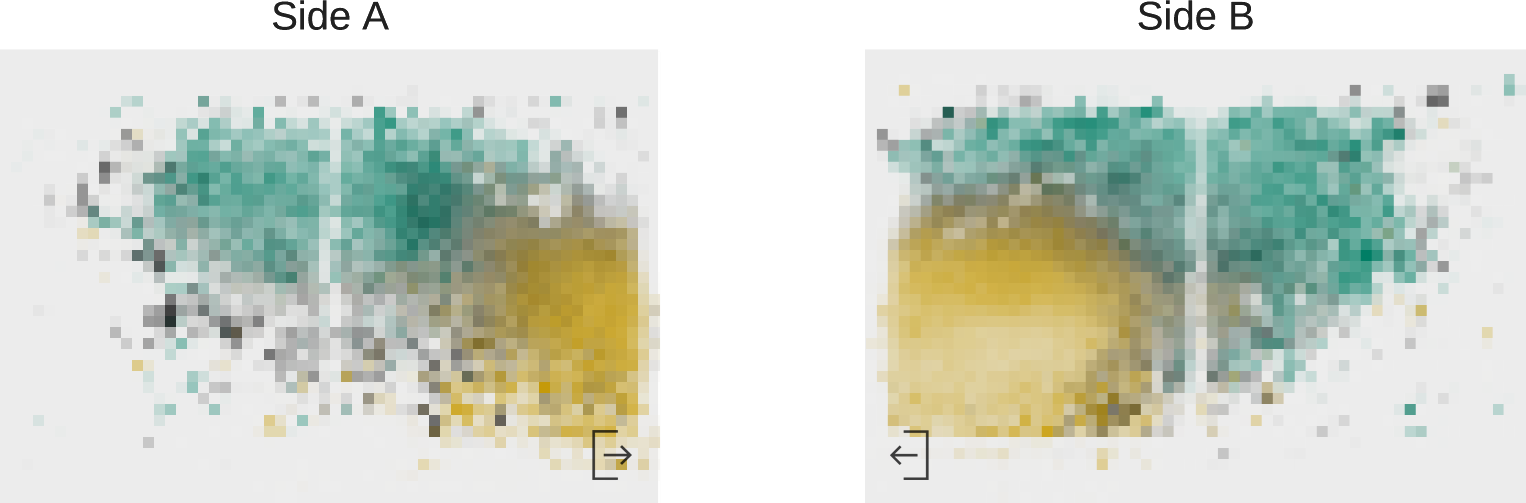
\includegraphics[width=1.0\textwidth]{Figures/wt_network3}
	\end{subfigure}
	
	\begin{subfigure}[b]{1.0\textwidth}
	\centering
	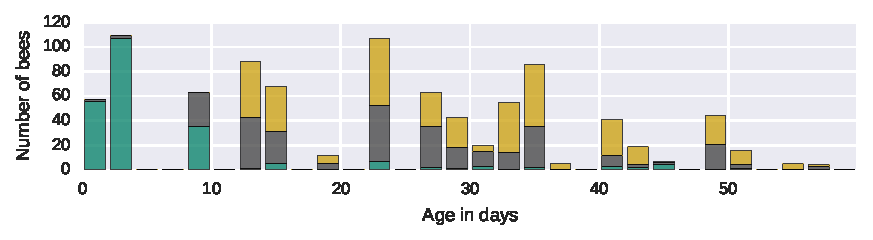
\includegraphics[width=1.0\textwidth]{Figures/n3-ageDistribution-WT}
	\caption[Walktrap communities]{Walktrap communities}
	\label{fig:n3ageWT}
	\end{subfigure}
	
	
	\caption[Age and spatial distribution of communities]{\textbf{Age and spatial distribution of communities} \emph{Green} represents the young community occupying the center area of the comb and \emph{orange} the old community, which is situated closer to the hive access. For walktrap the \emph{gray} middle-aged community is positioned between the other to and in the periphery of the comb.}
	\label{fig:n3-communities}
\end{figure}
\clearpage
\newpage
\section{Temporal Perspectives of Honey Bee Networks}

For all three snapshots, the same exponentially decay regarding the edge weights can be seen in figure~\ref{fig:statEdgeWeightDist}.
The analysis of snapshot~1 and 2 showed that the same characteristic distribution of degree, strength, lcc, betweenness, and closeness for snapshot~1~\ref{fig:n1-degreeStrLCC} and snapshot~2~\ref{fig:n2-degreeStrLCC} exists. They also follow a normal distribution and the characteristic bimodality is shown. The correlation between the local measure and detection frequency and age remains.
This shows that the characteristics described in section~\ref{subsubsec:bees} applies for all three snapshots and is, therefore, stable for this investigated time interval. A low hierarchical structure and the correlation with age and detection frequency seem to be a global property of the colony.

%%%%%%%%%%%%%%%%%%%%%%%%%%%%%%%%%%%%%%%%%%%%%%%%%%%%%%%%%%%%%%%%%%%%%%%%%%%%%%%
\subsection{Stability of Functional Groups}
%%%%%%%%%%%%%%%%%%%%%%%%%%%%%%%%%%%%%%%%%%%%%%%%%%%%%%%%%%%%%%%%%%%%%%%%%%%%%%%
Table~\ref{tab:communities} lists the exact number of bees per community for each algorithm and snapshot.
For each snapshot, the leading eigenvector detected two communities with about the same number of bees.
The first communities CY(1,2,3) contain the queen and on average younger bees than the second communities CO(1,2,3).\\
In comparison, walktrap identified three communities, but two for the first snapshot.
Again the first communities CY(1,2,3) consist of the queen and on average younger bees than the second CM(2,3) and third communities CO(1,2,3).
The bees in CM2 and CM3 are on average younger than the bees in CO2 and CO3.
Figure~\ref{fig:ageDistribution} depicts the age distribution for each community and snapshot.

A two-sample Kolmogorov–Smirnov test showed that the age distributions are significantly different ($p< 0.001$) for both algorithms. However, the $p$-values for the walktrap communities CM2, CO2, and CM3, CO3 are lower.
The spatial segregation of the communities is very similar in all three snapshots. For further reference see the heat maps in~\ref{fig:communitiesPerNetworkWT} and~\ref{fig:communitiesPerNetworkLE}.
The detected communities seem to differ in their respective age and occupy different areas of the comb, but remain stable over this inpected time interval.

\begin{table}
\centering
\caption[Overview about communities]{\textbf{Overview about communities per network} Communities marked with * contain the queen. Age and standard deviation (SD) are measured in days. For each network the queen and bees with a negative agre are excluded: network 1 - 12 bees, network 2 - 119 bees, network 3 - 10 bees.}
\label{tab:communities}
\vspace*{5mm}
\begin{tabular}{lcrrrrr}
	\toprule
	{}  & ID & Members & Proportion & Age & SD\\
	\midrule
	\rowcolor{Gray}
	Leading eigenvector &&&&&\\
	\midrule 
	\quad Network 1  & CY1 & $*430$  & 47.25\% & $17.12$ & $\pm10.97$ \\
	                 & CO1 & $480$   & 52.75\% & $27.24$ & $\pm10.96$ \\
	\midrule   							
	\quad Network 2  & CY2 & $*392$  & 45.63\% & $20.24$ & $\pm12.01$ \\
	                 & CO2 & $467$   & 54.37\% & $28.10$ & $\pm10.88$ \\
	\midrule  
	\quad Network 3  & CY3 & $*381$  & 41.78\% & $13.15$ & $\pm13.50$ \\
	                 & CO3 & $531$   & 58.22\% & $28.70$ & $\pm11.67$ \\
    \midrule
    \rowcolor{Gray}
    Walktrap &&&&&\\
    \midrule 
	\quad Network 1 & CY1 & $*427$ & 46.92\% & $17.07$ & $\pm10.92$\\
	                & CO1 & $482$  & 52.97\% & $27.23$ & $\pm11.00$\\
	\midrule
	\quad Network 2 & CY2 & $*263$ & 30.62\% & $18.23$ & $\pm11.46$\\
				    & CM2 & $305$  & 35.51\% & $25.20$ & $\pm11.47$\\
				    & CO2 & $291$  & 33.88\% & $29.47$ & $\pm10.06$\\            
	\midrule
	\quad Network 3 & CY3 & $*229$  & 25.11\% & $6.55$  & $\pm10.36$\\
					& CM3 & $298$  & 32.68\% & $25.08$ & $\pm11.97$\\
					& CO3 & $385$  & 42.21\% & $29.29$ & $\pm11.44$\\
	\bottomrule
\end{tabular}
\end{table}
\begin{table}
\centering
\caption[Kolmogorov-Smirnov test]{\textbf{Kolmogorov-Smirnov test} $p$-values for leading eigenvector (LE) and walktrap (WT) for each network and its communities.}
\label{tab:pvalues2}
\vspace*{5mm}
\begin{tabular}{lcrrrrr}
	\toprule

	\rowcolor{Gray}
	 & & LE p-value & WT p-value\\
	\midrule 
	\quad Network 1     & CY1, CO1 & 2.18e-33 & 1.52e-32 \\
	\midrule   							
	\quad Network 2     & CY2, CO2 & 2.99e-20 & 2.3e-32 \\
					    & CY2, CM2 &          & 4.72e-10\\
					    & CM2, CO2 &          & 1.00e-04\\
	\midrule  
	\quad Network 3     & CY3, CO3 & 5.10e-66 & 5.51e-67\\
					    & CY3, CM3 &          & 1.10e-95\\
						& CM3, CO3 &          & 1.98e-05\\ 
	\bottomrule
\end{tabular}
\end{table}

%%%%%%%%%%%%%%%%%%%%%%%%%%%%%%%%%%%%%%%%%%%%%%%%%%%%%%%%%%%%%%%%%%%%%%%%%%%%%%%
\subsection{Dynamic of Individual Bees}
%%%%%%%%%%%%%%%%%%%%%%%%%%%%%%%%%%%%%%%%%%%%%%%%%%%%%%%%%%%%%%%%%%%%%%%%%%%%%%%
Figure~\ref{fig:membersLE} (LE) and figure~\ref{fig:membersWT} (WT) show the flow of bees between consecutive snapshots and communities.
For leading eigenvector communities, the majority of bees stay in their age group, and a small fraction of bees switches to older communities.
Only a few bees change to younger communities.
The new middle-aged communities CM2 and CM3, detected by walktrap, consist partly of young (CY1) and old (CO1) bees. The switching behavior of individuals between communities is similar to leading eigenvector.
Individual bees change communities as they age.

\begin{figure}[htb]
	\centering
	\begin{subfigure}[b]{0.49\textwidth}
	\centering
	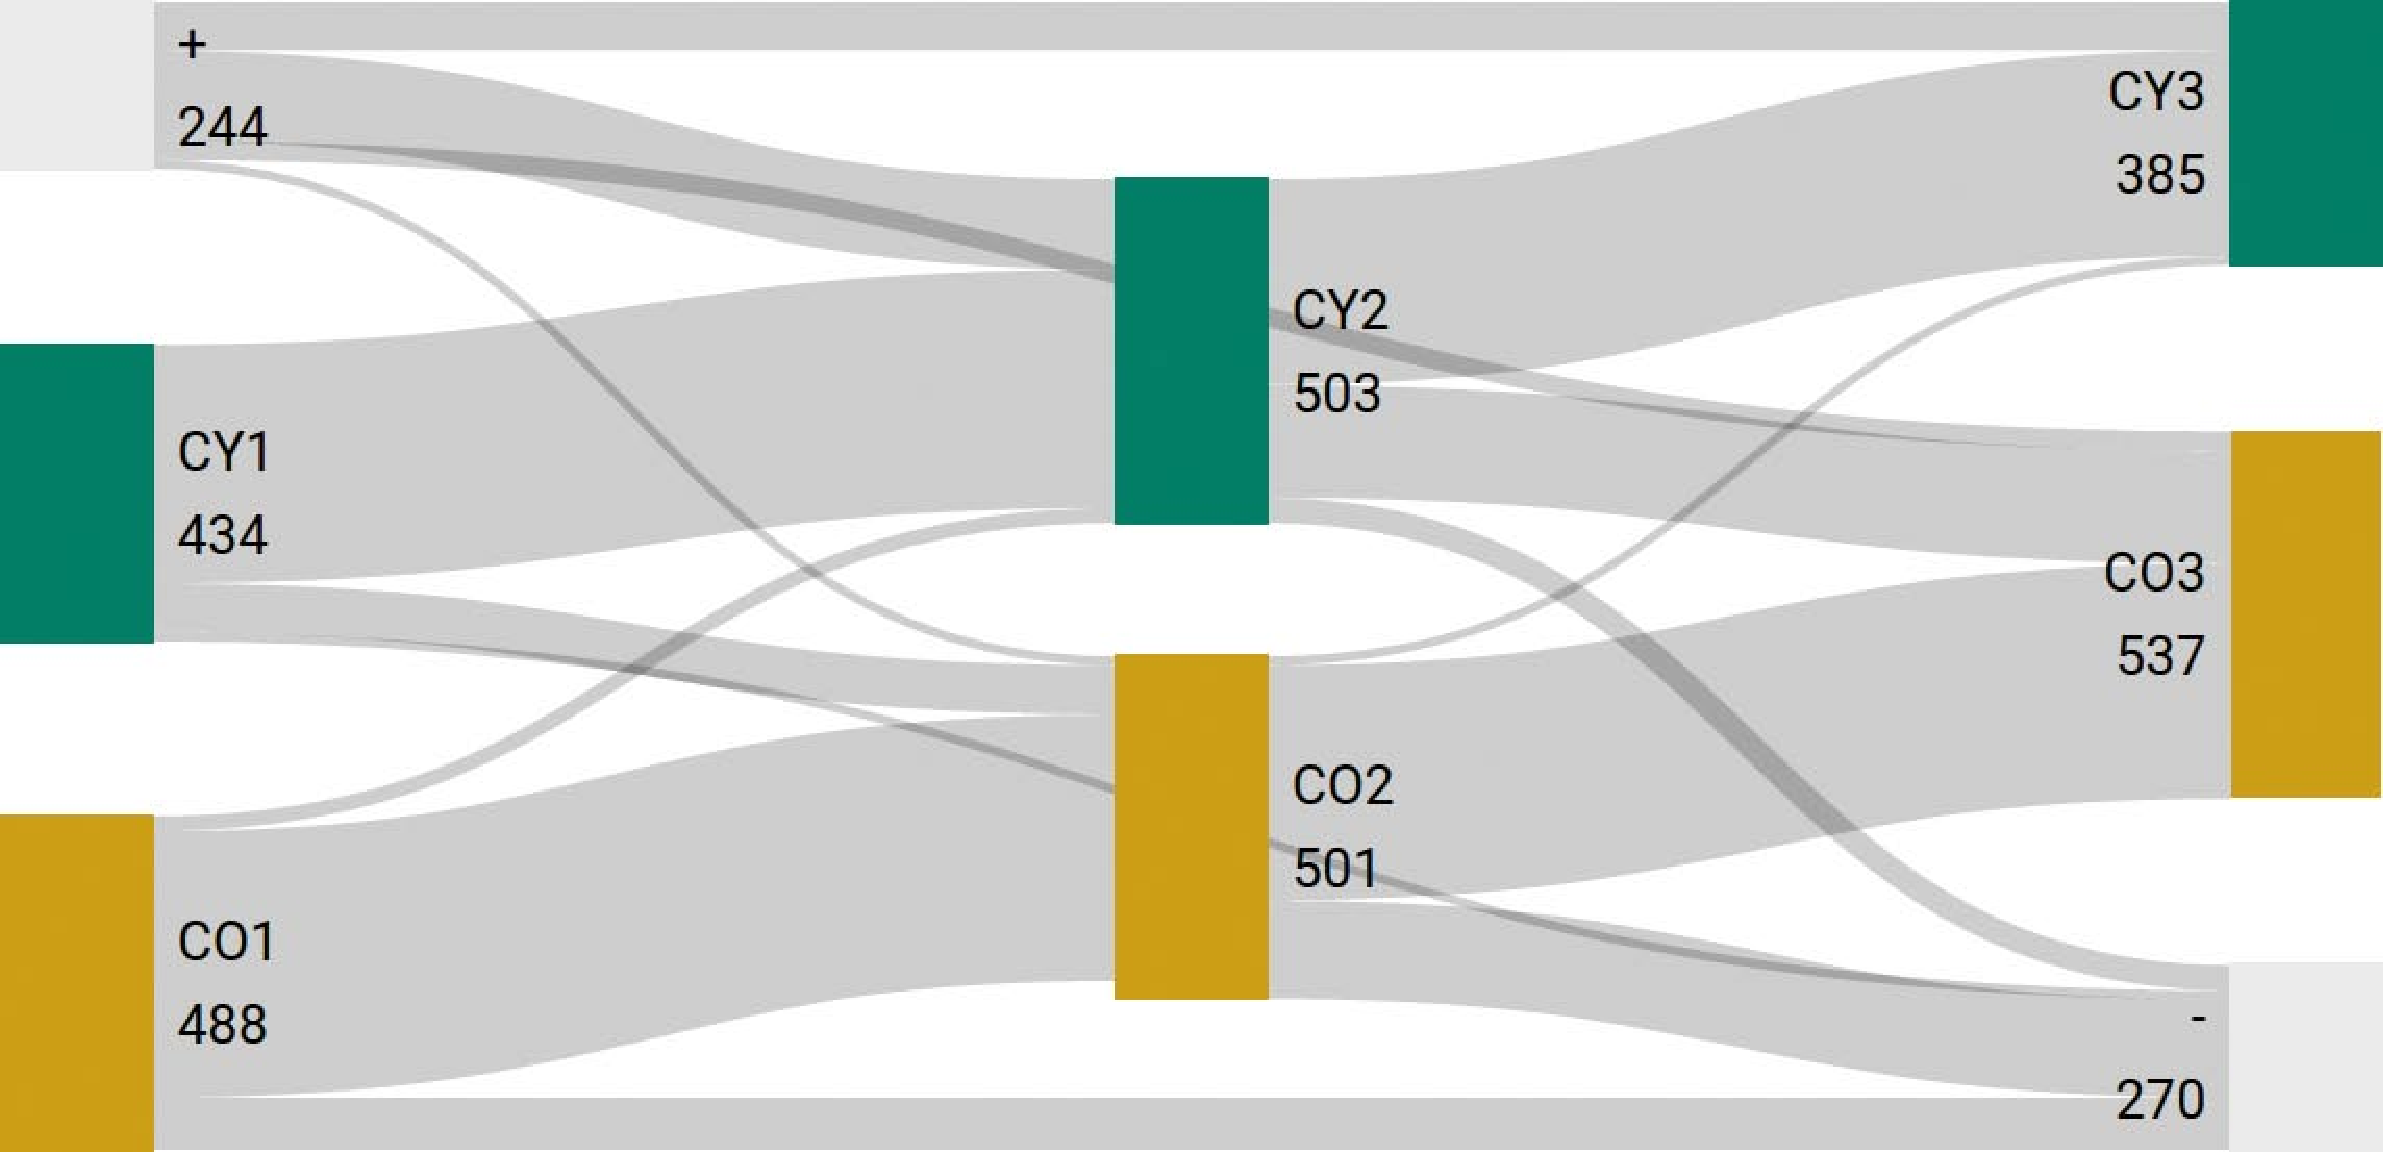
\includegraphics[width=0.95\textwidth]{Figures/LE_matching}
	\caption[Leading eigenvector communities]{Leading eigenvector communities}
	\label{fig:membersLE}
	\vspace*{5mm}
	\end{subfigure} 
	\begin{subfigure}[b]{0.49\textwidth}
	\centering
	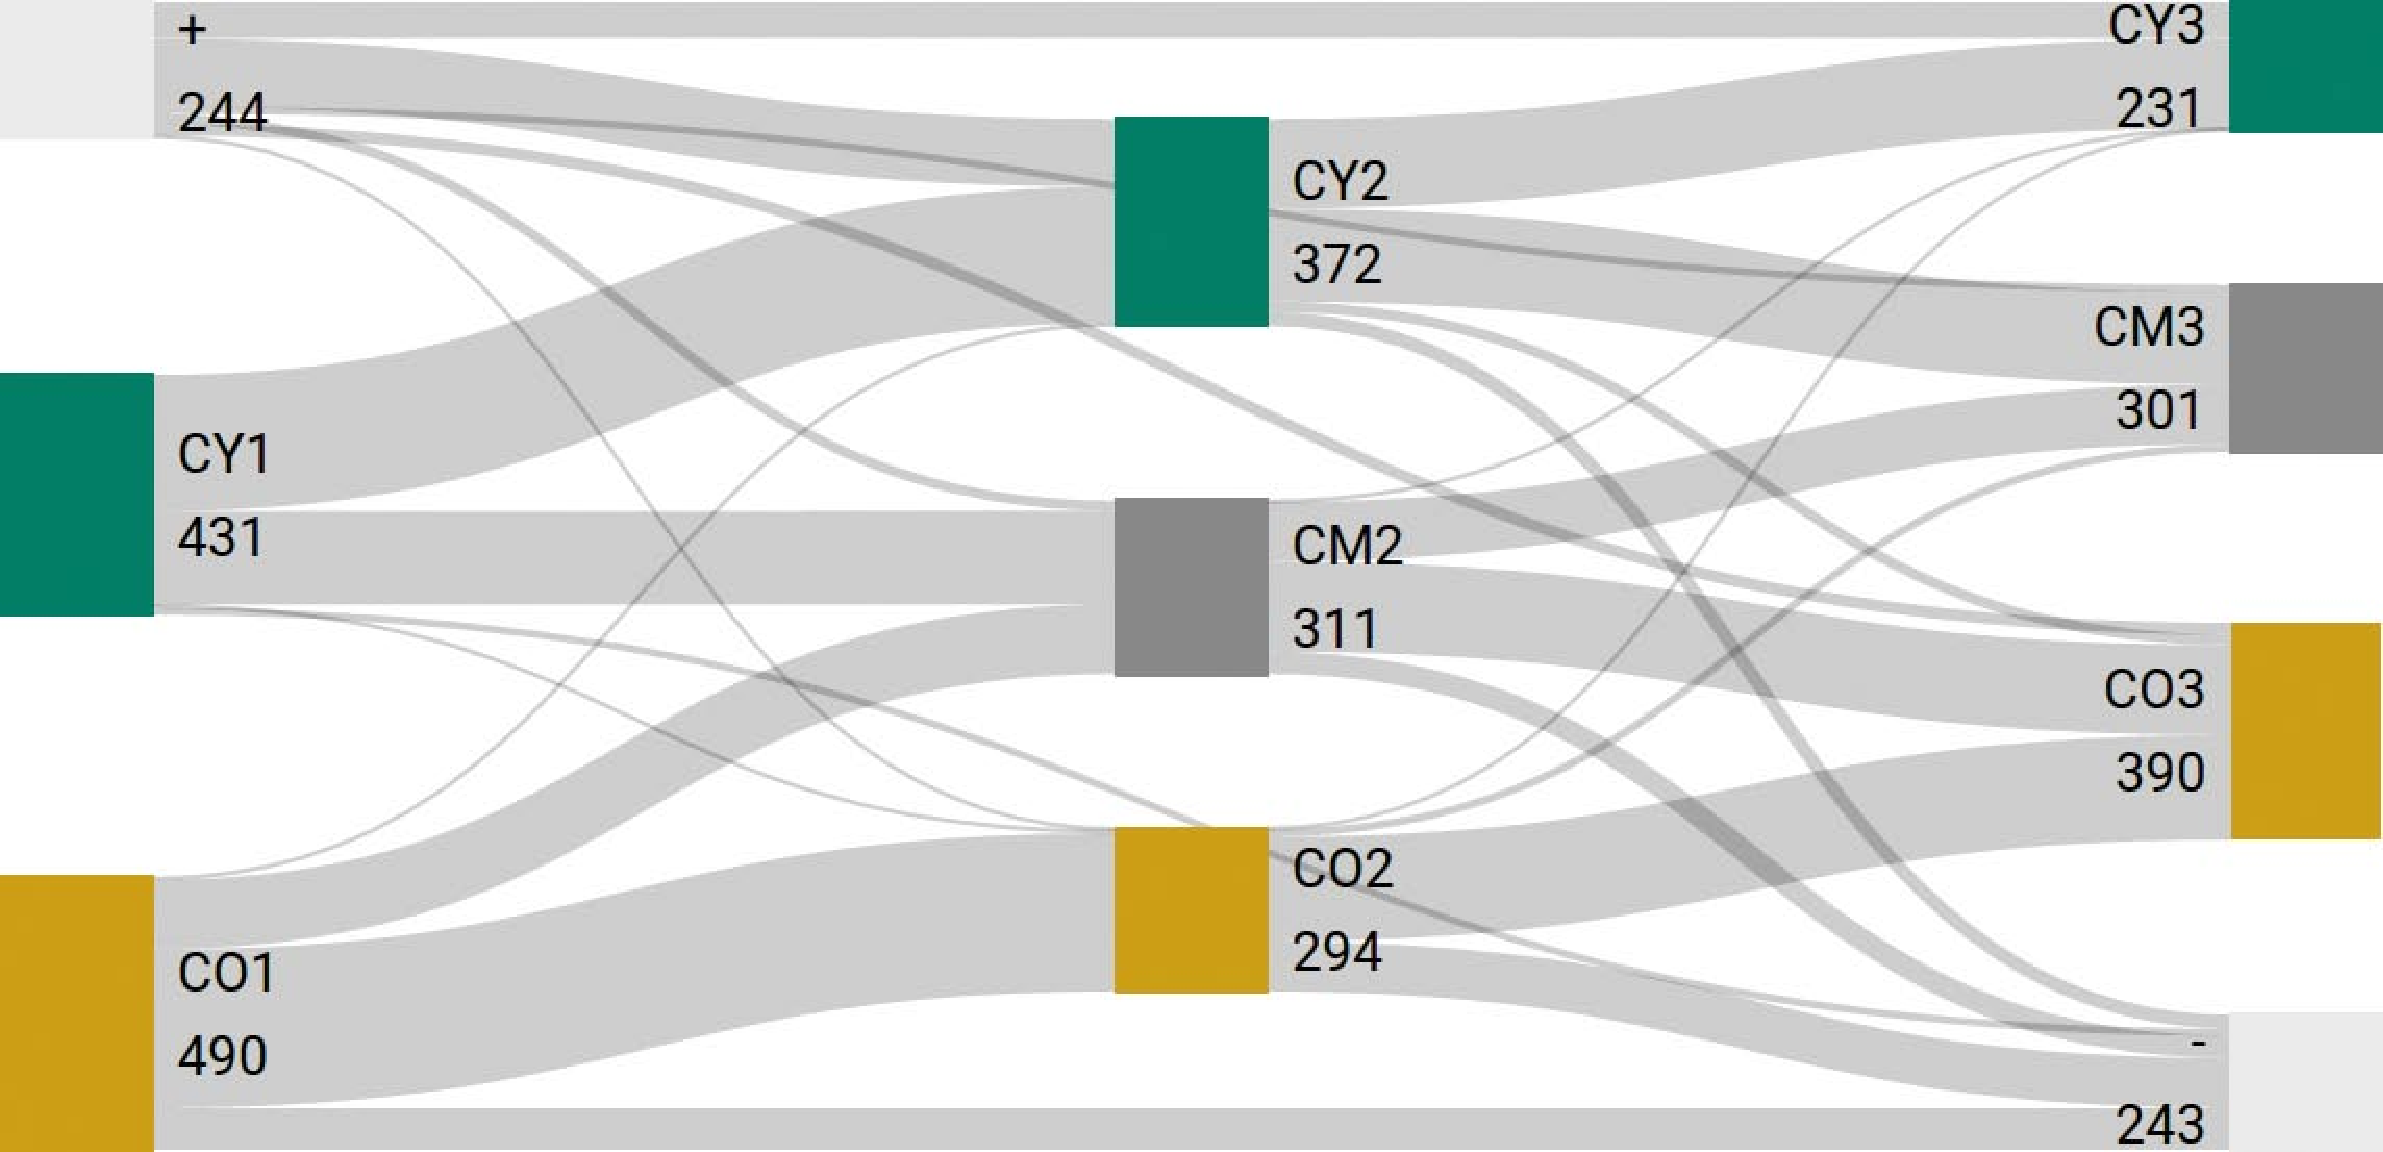
\includegraphics[width=0.95\textwidth]{Figures/WT_matching}
	\caption[Walktrap communities]{Walktrap communities}
	\label{fig:membersWT}
	\vspace*{5mm}
	\end{subfigure}
	\caption[Dynamics of bees]{\textbf{Dynamics of bees} 
	Each column represents a time step, the colored rectangles represent the communities for each step, and the height of the rectangles corresponds to the number of its community members, as referenced by the number. \emph{Green} indicates the community containing young bees and the queen, \emph{gray} represents the community containing middle-aged bees (only for WT), and \emph{orange} the community containing old bees. This figure shows that the major part of the bees either stays in the same aged community or switch to an older group.}
	\label{fig:members}
\end{figure}

%%%%%%%%%%%%%%%%%%%%%%%%%%%%%%%%%%%%%%%%%%%%%%%%%%%%%%%%%%%%%%%%%%%%%%%%%%%%%%%
%%%%%%%%%%%%%%%%%%%%%%%%%%%%%%%%%%%%%%%%%%%%%%%%%%%%%%%%%%%%%%%%%%%%%%%%%%%%%%%
\section{Discussion of Results}
%%%%%%%%%%%%%%%%%%%%%%%%%%%%%%%%%%%%%%%%%%%%%%%%%%%%%%%%%%%%%%%%%%%%%%%%%%%%%%%
%%%%%%%%%%%%%%%%%%%%%%%%%%%%%%%%%%%%%%%%%%%%%%%%%%%%%%%%%%%%%%%%%%%%%%%%%%%%%%%

In the following chapter, I summarize and discuss my results considering the current state of research.
This part is structured according to the research goals, listed in Section~\ref{sec:intro:goals}.
First I discuss the topology of the spatial proximity networks of honey bees and its characteristic properties.
Secondly, I compare the observed communities and their development over time with existing theories regarding temporal polyethism.


%%%%%%%%%%%%%%%%%%%%%%%%%%%%%%%%%%%%%%%%%%%%%%%%%%%%%%%%%%%%%%%%%%%%%%%%%%%%%%%
\subsection{Network Topology and Properties of Honey Bee Colonies}
%%%%%%%%%%%%%%%%%%%%%%%%%%%%%%%%%%%%%%%%%%%%%%%%%%%%%%%%%%%%%%%%%%%%%%%%%%%%%%%
The honey bee spatial proximity networks are characterized by a high density (69\%, 54\%, 61\%), which means the bees encounter many nestmates during the ten hours of data aggregation.
This results either from high activity or the fact that the comb is simply very full.
The latter increases the probability that two bees are close to each other.\\
Comparing this result to the ant contact networks of Mersch~et~al.\cite{mersch2013tracking}~($D=72\%\pm5.3$), the values are similar.
In contrast, when compared to \textcite{baracchi2014socio}~($D=0.15$) the density is higher, probably due to their lower observation resolution of one frame per minute.


The small diameter~($d_{\texttt{max}}=3$) of my investigated networks and the low average shortest path of~$1.4$ in combination with a high global clustering coefficient~($0.79$, $0.72$, $0.75$) are characteristic for a class of networks known as small-world networks.
This type of networks allows for rapid and efficient communication between individuals.


\textcite{charbonneau2013social} state that it is assumed that many biological networks, including insect colonies, approximate scale-free networks.
For some of them, the scale-free property has been shown, but for social insect networks this question remains open.
Investigated social insect colonies are often small and therefore the methods for the recognition of scale-free phenomena are limited.
They do not specify the type of social insect networks, whether the inference of interactions is based on spatial proximity, physical contacts, or food transfer events.\\
The network I explored is large compared to past studies (Section ~\ref{ch:relatedwork}). The degree distribution of the investigated spatial proximity network of honey bees does not follow a power-law;
the absence of hubs and a non-hierarchical structure characterizes this network.
This result corresponds to the decentralized structure of a honey bee colony, and the absence of a central authority described by Seeley~\cite{seeley1989honey}.


I noticed bimodal degree, strength, closeness and betweenness distributions and a right skewed lcc distribution, corresponding mainly to bees older than~45~days.
While inspecting this group of bees, I found that this group has a very low detection rate and is not part of any other following snapshot.
Probably this group of bees dies during that day.
Bees who are present in the hive earlier that day and are then absent for the rest of the day have very low network measure values.
The total number of old bees is relatively small compared to other age groups.
Consequently, low network measure values strongly affect the mean of that old group and should be excluded in future studies.


Generally, I observed a correlation between the detection frequency of a bee, its age, and its corresponding network measure value.
Older bees are detected less often than younger bees and therefore differ in their network measures.
The age-based task division of bees in a colony observed by \textcite{seeley1989social} might be an explanation; namely, old bees are foragers, the middle-aged bees conduct several tasks inside the hive but mainly they store resources, and young bees are primarily nursing.
\textcite{baracchi2014socio} also assumed that the time which bees spend outside the hive probably affects their connectedness within the interaction network.

%%%%%%%%%%%%%%%%%%%%%%%%%%%%%%%%%%%%%%%%%%%%%%%%%%%%%%%%%%%%%%%%%%%%%%%%%%%%%%%
\subsection{Characterization of Functional Groups and its Dynamics}
%%%%%%%%%%%%%%%%%%%%%%%%%%%%%%%%%%%%%%%%%%%%%%%%%%%%%%%%%%%%%%%%%%%%%%%%%%%%%%%
According to the definition of communities in Section~\ref{subsec:bg:communities}, I found two to three communities, depending on the algorithm applied.

The algorithms (LE and WT) detected communities, despite a high network density and without thresholding links of low values, as opposed to~\textcite{mersch2013tracking}.
The authors reduced the network's density artificially to 25\% to apply the infomap algorithm.

I also examined the spatial fidelity of the revealed communities and their age composition, similar to \textcite{baracchi2014socio}.
I found that younger bees are located close to the brood (upper center of the comb); older bees are situated closer to the hive exit, and middle-aged bees are placed between the two groups and around the brood, where the cells for honey storage are located.

I inspected three snapshots over a period of five days and found that the detected communities are stable over time.
Age-division and spatial fidelity can be observed in all the snapshots.
Bees from younger communities move to older communities as they age. Only a few bees changed from older to younger communities.

It is surprising that my results align with \textcite{baracchi2014socio}, because they did not use a community detection algorithm.
The authors conducted a hierarchical clustering based on the network measures strength, eigenvector and betweenness centrality of individual bees.
Moreover, their colony contained bees of three predetermined age cohorts, instead of representing all age groups ranging from 0 to 60 days, as in my study.

The communities I detected are similar to the groups of bees formed by temporal polyethism.
The old bees positioned closer to the hive exit may be the foragers, the middle-aged group spatially close to the storage cells may be the food storage bees and the group of young bees  may be the cell cleaning and brood care bees because they are located close to the brood. My findings are very close to the ones of \textcite{baracchi2014socio}.

The two approaches discovered the same functional groups of the bee colony, on the one hand by node level network measures (hierarchical clustering) and on the other hand by a higher than expected density of nodes (community detection).
That acknowledges the existence of the age-based division of labor in honey bee colonies as well as the higher communication frequency within groups than between groups.
Nevertheless, the low modularity score indicates that the segregation of groups is not that obvious and strict; therefore a lot of interaction between groups exists.

\textcite{mersch2013tracking} revealed that the behavioral maturation of ants is a slow and noisy process. Instead of investigating the transition of individuals day wise, they grouped 41 days in four periods. For each period they assigned each ant to a community if it was found in this community 70\% of the time.
It seems that honey bee transitions are in contrast to ants faster and smoother.